\documentclass[12pt]{article}

\usepackage[spanish]{babel}
\usepackage[utf8]{inputenc}
\usepackage{graphicx}
\usepackage{geometry}
\usepackage{xcolor}
\usepackage{fancyhdr}
\usepackage{lastpage}
\usepackage{pdfpages}
\usepackage{listings}

\geometry{top=25mm,left=15mm,right=15mm,a4paper}

\pagestyle{fancy}
\fancyhf{}
\lhead{Sistemas Operativos}
\cfoot{Página \thepage\ de \pageref{LastPage}}

\graphicspath{./}

\begin{document}
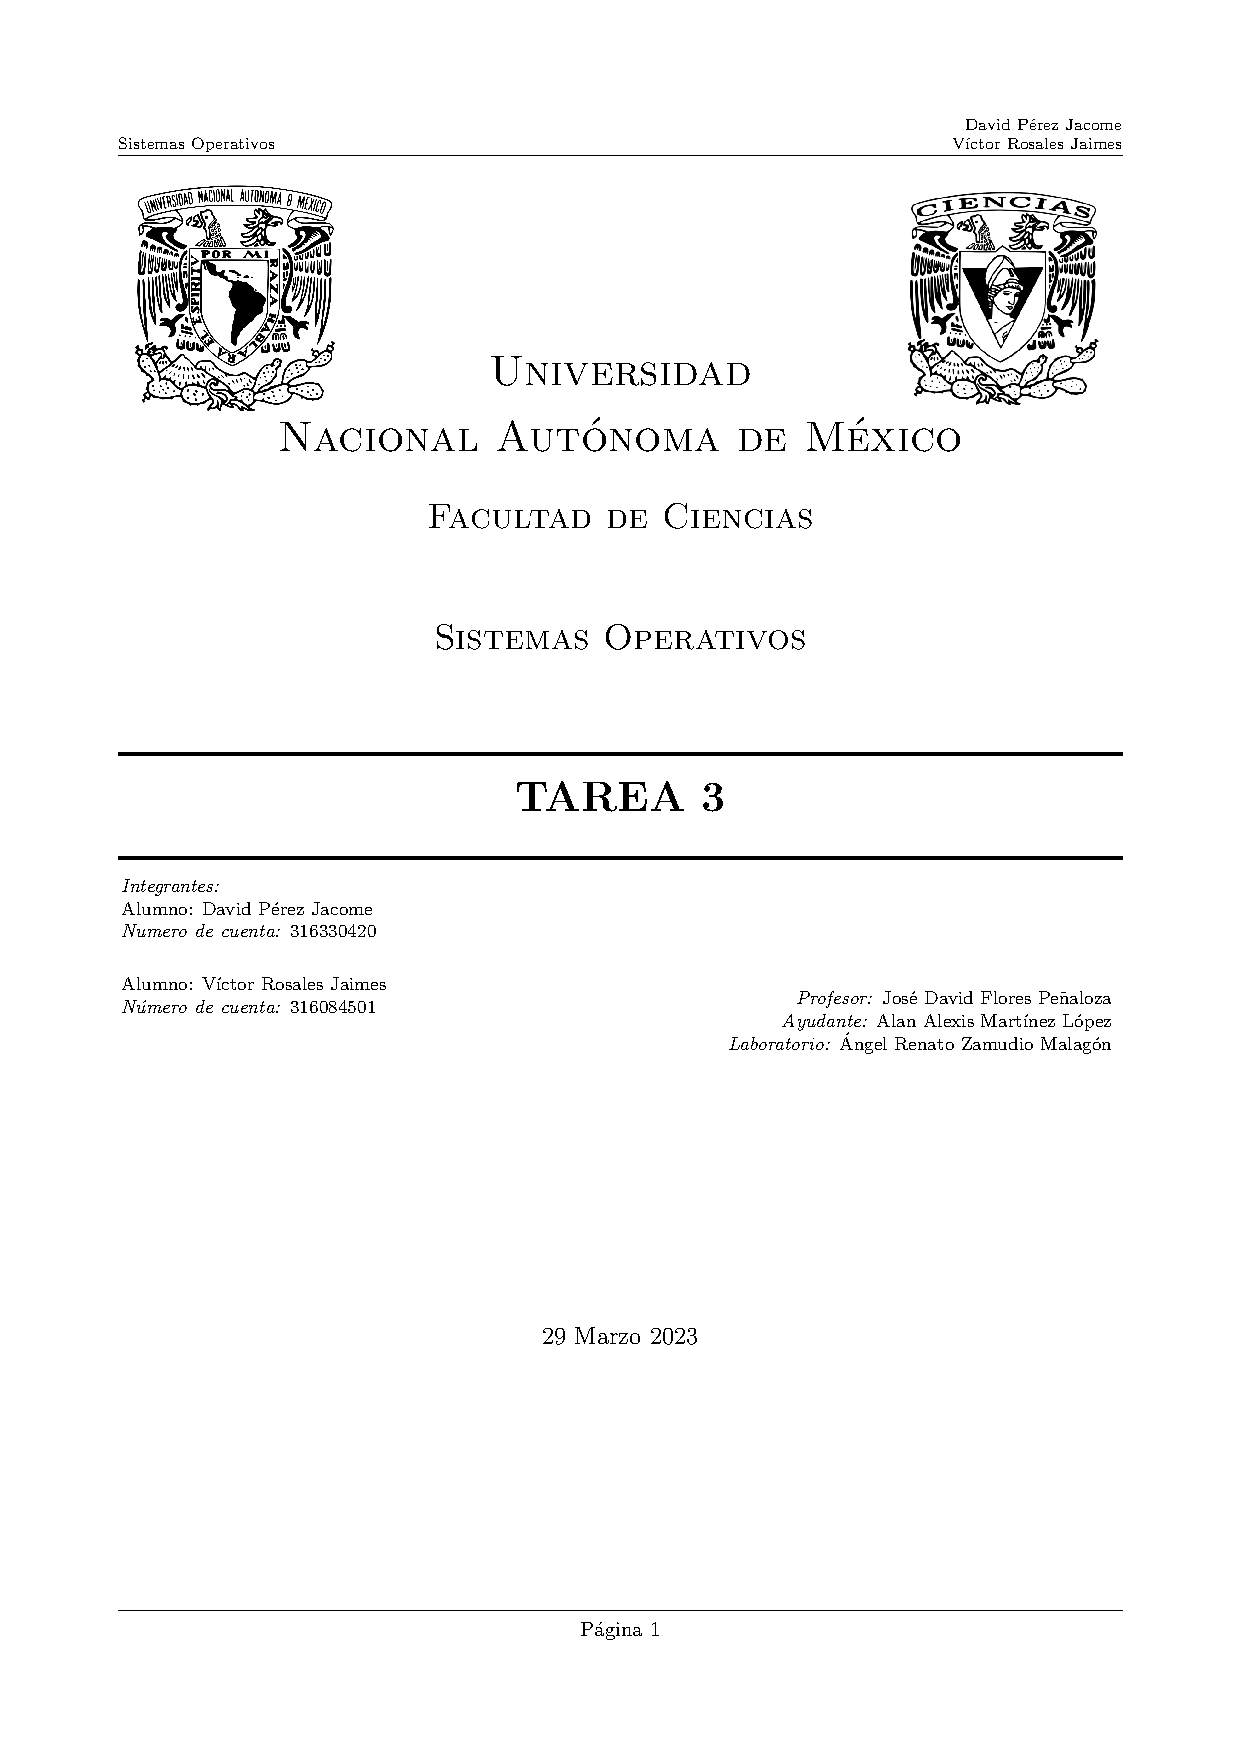
\includepdf{Portada.pdf}
{\color{blue} \section*{Tarea 3.}}

{\color{blue} \subsection*{Instrucciones.}}
\vspace{0.5em} 

Lee con atención las preguntas y contesta lo correspondiente. La tarea se entregará por vía classroom
en un archivo pdf que debe tener el nombre completo y número de tarea, ya sea en una portada o en el encabezado.
\textbf{La tarea se entregará de manera individual.}\\

{\color{blue} \subsection*{Ejercicios}}
\vspace{0.5em}

\begin{enumerate}
    \item Menciona y describe las 3 formas de pasar los parametros a una llamada al sistema.
    \vspace{2mm}

    \textbf{RESPUESTA.}

    \item ¿Qué elementos debe contener un Boque de control de procesos(BCP)?
    \vspace{2mm}
    
    \textbf{El bloque de control de proceso es una tabla que administra las caracteristicas de un proceso y principalmente debe de tener: 
    \begin{enumerate}
        \item Estado.
        \item Información.
    \end{enumerate}}
    
    \item ¿Qué es el descriptor de hardware del proceso?
    \vspace{2mm}

    \textbf{RESPUESTA.}

    \item ¿Por qué es necesario que exista un descriptor de hardware del proceso?
    \vspace{2mm}

    \textbf{RESPUESTA.}

    \item Si tenemos un BCP por cada proceso ¿Cómo tenemos control de todos ellos?
    \vspace{2mm}

    \textbf{RESPUESTA.}

    \item ¿Qué es, como se le dice y cuáles son las caracteristicas y tareas del manejador de interrupciones de primer nivel?
    \vspace{2mm}

    \textbf{RESPUESTA.}
    \item ¿Cómo se determina de donde viene una interrupción?  
    \vspace{2mm}

    \textbf{RESPUESTA.}

    \item ¿Qué es y que hace una Skip chain?
    \vspace{2mm}

    \textbf{RESPUESTA.}
    
    \item Explica cuáles son las tareas del despachador.
    \vspace{2mm}

    \textbf{RESPUESTA.}

    \item Explica cuáles son las tareas del calendarizador.
    \vspace{2mm}
    
    \textbf{RESPUESTA.}

    \item ¿Qué es la concurrencia real y concurrencia aparente? 
    \vspace{0mm}
    \textbf{\begin{enumerate}
        \item Concurrencia Real: Cada proceso se ejecuta en un solo procesador.
        \item Concurrencia Aparente: Concurrencia emulada ya que se corren varios hilos en un procesador.
    \end{enumerate}}

    \item ¿Qué es el no-determinismo?
    \vspace{2mm}
    
    \textbf{RESPUESTA.}

    \item ¿Qué es un programa o rutina?
    \vspace{2mm}
    
    \textbf{RESPUESTA.}

    \item ¿Qué es un procesador y cuál es su función?
    \vspace{2mm}
    
    \textbf{RESPUESTA.}

    \item ¿Qué es un semáforo y para qué sirve?
    \vspace{2mm}
    
    \textbf{RESPUESTA.}

    \item Explica con tus palabras que es Exclusión Mutua.
    \vspace{2mm}
    
    \textbf{RESPUESTA.}

    \item Explica con tus palabras que es Deadlock (interbloqueo).
    \vspace{2mm}
    
    \textbf{RESPUESTA.}

    \item Explica con tus palabras que es Hambruna.
    \vspace{2mm}
    
    \textbf{RESPUESTA.}

    \item Explica con tus palabras que es Sección Critica.
    \vspace{2mm}
    
    \textbf{RESPUESTA.}

    \item Explica con tus palabras que son las condiciones de competencia.
    \vspace{2mm}
    
    \textbf{RESPUESTA.}

    \item Explica con tus palabras que es la sincronización en cuánto a concurrencia.
    \vspace{2mm}
    
    \textbf{RESPUESTA.}

    \item ¿Por qué la implementación de \textbf{wait} tiene que tener acceso directo al despachador de procesos?
    \vspace{2mm}
    
    \textbf{RESPUESTA.}

\end{enumerate}

\end{document}